% Full technical report. Build:
%   python ../scripts/generate_report_latex_data.py
%   python ../scripts/build_report_figures.py   % optional; needs artifacts/benchmark_summary.json
%   ../.tools/tectonic/tectonic full_report.tex
% Or use pdflatex after installing TeX Live.
\documentclass[11pt,a4paper]{article}
\usepackage[margin=2.3cm]{geometry}
\usepackage{graphicx}
\usepackage{booktabs}
\usepackage{amsmath}
\usepackage{microtype}
\usepackage[hidelinks]{hyperref}
\usepackage{url}
\usepackage{tikz}
\usetikzlibrary{arrows.meta,positioning}

\title{\textbf{Aqueous diffusion coefficients from structure and temperature}\\[0.4em]
\large Reproducible pipeline on Han et al.\ supporting data (Table~S2)}
\author{Technical report (codebase \texttt{diffusion-mol})}
\date{\today}

%% AUTO-GENERATED by scripts/generate_report_latex_data.py — do not edit


\newcommand{\GeneratedDataTable}{%
\begin{tabular}{@{}lr@{}}
\toprule
Quantity & Value \\
\midrule
Rows after cleaning & 20,576 \\
Unique SMILES & 6,909 \\
$T$ range in data (K) & 273.75 -- 394.0 \\
Invalid SMILES dropped & 0 \\
Duplicate $(\text{SMILES},T)$ collapsed & 152 (mean $D$) \\
\bottomrule
\end{tabular}
}

\newcommand{\GeneratedBenchmarkTable}{%
\begin{tabular}{@{}llccc@{}}
\toprule
Split & Model & RMSE $\log_{10}D$ & $R^2$ & Med.\ $| \hat D-D|/D$ \\
\midrule
Random & Mean $\log_{10}D$ & 0.4731 & -0.000 & 0.7910 \\
Random & Median $\log_{10}D$ & 0.4938 & -0.089 & 0.7750 \\
Random & Ridge (FP+T) & 0.1068 & 0.949 & 0.1293 \\
Random & MLP & 0.1028 & 0.953 & 0.1105 \\
Random & GNN & 0.0989 & 0.956 & 0.1026 \\
\midrule
Scaffold & Mean $\log_{10}D$ & 0.4708 & -0.000 & 0.7898 \\
Scaffold & Median $\log_{10}D$ & 0.4915 & -0.090 & 0.7666 \\
Scaffold & Ridge (FP+T) & 0.1065 & 0.949 & 0.1379 \\
Scaffold & MLP & 0.0843 & 0.968 & 0.1006 \\
Scaffold & GNN & 0.0766 & 0.974 & 0.1020 \\
\bottomrule
\end{tabular}
}

\newcommand{\GeneratedHyperparamTable}{%
\begin{tabular}{@{}lr@{}}
\toprule
Setting & Value \\
\midrule
Train / val / test fraction & 0.70 / 0.15 / 0.15 \\
Split RNG seed & 42 \\
Morgan radius / bits & 2 / 2048 \\
Batch size / max epochs / patience & 128 / 200 / 25 \\
Optimizer / LR / weight decay & AdamW / 0.001 / 1e-05 \\
Loss & Huber ($\delta=1.0$) on $\log_{10} D$ \\
MLP hidden dims / dropout & [512, 256, 128] / 0.2 \\
GNN (GINE) hidden dim / layers / dropout & 128 / 4 / 0.2 \\
\bottomrule
\end{tabular}
}


\begin{document}
\maketitle

\begin{abstract}
Predicting the aqueous diffusion coefficient $D$ as a function of molecular structure and temperature is an underdetermined physics-informed learning problem when only experimental tables are available. This report documents an implemented pipeline: load and clean the supplemental spreadsheet \texttt{jp5c01881\_si\_002.xlsx}, regress $\log_{10} D$ with train-only temperature standardization, and evaluate on molecule-level held-out sets including a Bemis--Murcko scaffold split. We compare fingerprint multilayer perceptrons, graph neural networks (GINE), and linear and trivial baselines. The best configuration in our runs (GNN, scaffold test) reaches test $R^2 \approx 0.97$ on $\log_{10} D$ and median relative error $\approx 0.10$ on $D$, far below constant baselines. Scope is \textbf{water only}; absolute $D$ requires confirming units against the primary publication.
\end{abstract}

\tableofcontents
\newpage

\section{Introduction}
\subsection{Goal}
The scientific target is to estimate \emph{aqueous} diffusion coefficients for small molecules given a SMILES string and temperature in kelvin. Applications include screening and interpreting transport in dilute aqueous environments. Pure curve fitting on $(\text{SMILES}, T) \mapsto D$ is only meaningful if evaluation respects chemical identity: the same compound must not appear in both training and test under different temperatures unless the task is explicitly row-level interpolation (which inflates scores).

\subsection{Relation to prior work}
The dataset used here is Table~S2 in the ACS supporting information file \texttt{jp5c01881\_si\_002.xlsx}, associated with work on learning diffusion in water from multimodal inputs. This \textbf{report does not reimplement or reproduce} the authors' published architecture; it describes an independent baseline stack (fingerprints + MLP, RDKit graphs + GINE) and transparent splits for comparison.

\section{Problem formulation}
\subsection{Target scale}
$D$ varies over many orders of magnitude. Direct mean-squared error on $D$ emphasizes large values. Following standard practice in property regression, we predict
\[
y = \log_{10} D, \qquad D = 10^{y},
\]
and optimize a robust loss on $y$ (Huber). Metrics are reported on $y$ (primary) and on back-transformed $D$.

\subsection{Conditional variable}
Temperature $T$ is kept in kelvin for physical consistency, then \textbf{z-scored using training-set mean and variance only} and applied unchanged at validation, test, and inference (\texttt{TemperatureScaler} wrapping \texttt{sklearn.preprocessing.StandardScaler}).

\subsection{Metrics}
For vectors $y_i$ (true log prediction) and $\hat{y}_i$:
\begin{itemize}
  \item MAE and RMSE on $\log_{10} D$.
  \item $R^2$ on $\log_{10} D$.
  \item MAE and RMSE on linear $D$ after $10^{y}$.
  \item Median of $\lvert \hat{D} - D\rvert / D$ over test points with $D>0$ (robust ``typical'' relative error).
\end{itemize}

\section{Data source and preprocessing}
\subsection{Source}
\begin{itemize}
  \item \textbf{File:} \texttt{jp5c01881\_si\_002.xlsx}.
  \item \textbf{Sheet:} \texttt{Table S2} (caption row + header row; loader uses \texttt{header=1}).
  \item \textbf{Columns:} \texttt{SMILSES} (workbook typo) $\rightarrow$ SMILES, \texttt{Temperature} (K), \texttt{D}. Auxiliary metadata columns are retained through cleaning where applicable.
\end{itemize}

\subsection{Cleaning policy}
\begin{itemize}
  \item Parse and \textbf{canonicalize} SMILES with RDKit; drop invalid rows (counted in the data report).
  \item \textbf{Deduplicate} $(\text{canonical SMILES}, T)$: aggregate duplicate $D$ by the \textbf{mean}; document pair count in the report.
\end{itemize}

\subsection{Dataset summary}
Table~\ref{tab:data} summarizes the cleaned table used for modeling.

\begin{table}[ht]
  \centering
  \caption{Cleaned dataset (after deduplication).}
  \label{tab:data}
  \GeneratedDataTable
\end{table}

\section{Methods}
\subsection{Molecule-level splits}
All splits assign every row of a given SMILES to exactly one of train, validation, or test (\textbf{no row-level leakage}).

\paragraph{Random split.} Unique SMILES are shuffled (seeded RNG) and partitioned 70\,/\,15\,/\,15.

\paragraph{Scaffold split.} Bemis--Murcko scaffolds are computed in RDKit; each scaffold is assigned wholly to one split; molecules inherit their scaffold's partition. Test scaffolds are unseen in training---a stricter probe of generalization to new chemotypes than random-by-molecule splits.

\subsection{Baselines}
\begin{itemize}
  \item \textbf{Mean / median} of training $\log_{10} D$ (constant predictors on the test set).
  \item \textbf{Ridge regression} on concatenated Morgan fingerprint and scaled $T$ (\path{sklearn.linear_model.Ridge}, $\alpha=1$).
\end{itemize}

\subsection{Molecular representations}
\paragraph{Fingerprints.} Morgan circular fingerprints (radius and bit width from config; default 2 / 2048), binary vectors from RDKit.

\paragraph{Graphs.} Hydrogen-added RDKit molecules are converted to PyG \texttt{Data} graphs. Node features: scaled atomic number, degree, formal charge, H count, aromaticity, ring flag, hybridization one-hot. Edge features: one-hot bond order (single, double, triple, aromatic).

\subsection{Models}
\paragraph{MLP.} Fully connected network on $\text{concat}(\text{FP}, T_{\text{scaled}})$ with ReLU, dropout, and linear readout to $\log_{10} D$.

\paragraph{GNN.} Stack of \texttt{GINEConv} layers (edge-conditioned message passing) with ReLU and dropout. Graphs are pooled with \path{global_mean_pool}, concatenated with $T_{\text{scaled}}$, and passed through an MLP head to $\log_{10} D$.

\subsection{Training protocol}
AdamW, Huber loss on $\log_{10} D$, weight decay, early stopping on \textbf{validation} Huber loss (patience 25, up to 200 epochs, batch 128). The best validation checkpoint is restored before testing. Saved weights include the temperature scaler for deployment.

\subsection{Software}
Python~3.10+, PyTorch, PyTorch Geometric, RDKit, scikit-learn, pandas. Defaults live in \path{configs/default.yaml}. Hyperparameters for the reported run appear in Appendix~\ref{app:hp}.

\section{Results}
\subsection{Quantitative comparison}
Table~\ref{tab:bench} lists held-out \textbf{test} metrics for both split protocols. Neural models strongly outperform trivial predictors and modestly improve over ridge on fingerprints.

\begin{table}[ht]
  \centering
  \caption{Test-set benchmarks (lower RMSE / higher $R^2$ better; median relative error on linear $D$).}
  \label{tab:bench}
  \small
  \GeneratedBenchmarkTable
\end{table}

\subsection{Figures}
Figure~\ref{fig:cmp} contrasts RMSE and $R^2$ in log space; Figure~\ref{fig:med} summarizes median relative error on $D$.

\begin{figure}[ht]
  \centering
  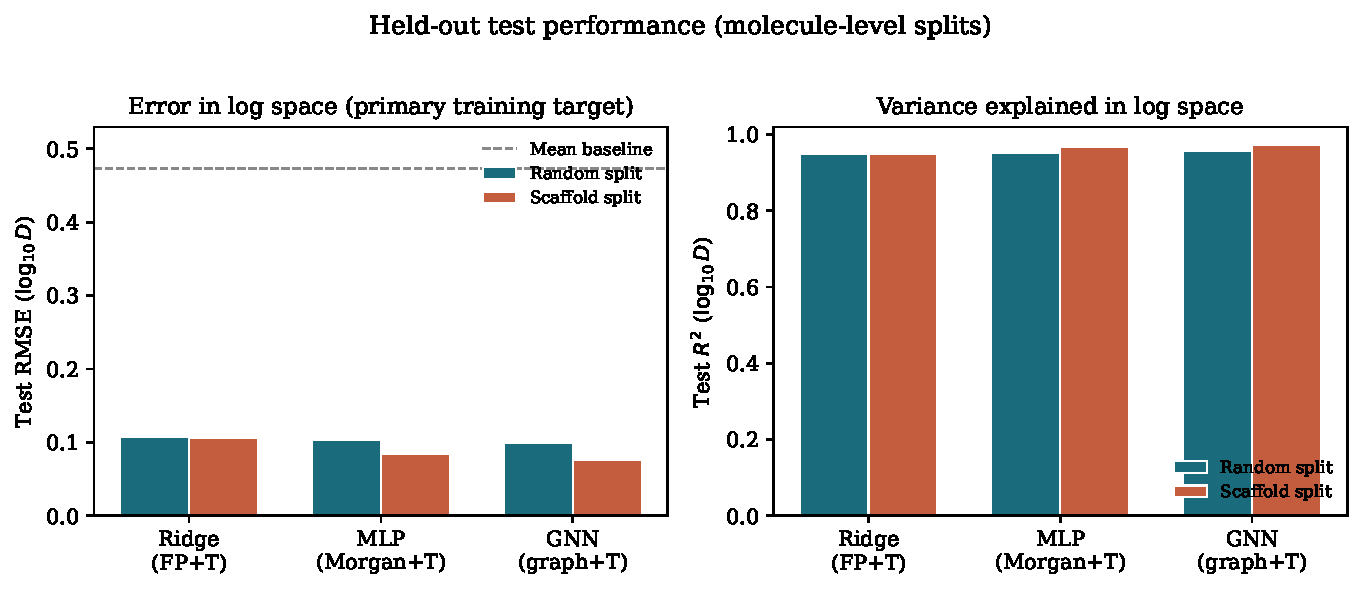
\includegraphics[width=\linewidth]{figures/model_comparison.pdf}
  \caption{Test RMSE and $R^2$ on $\log_{10} D$; dashed line: mean-$\log_{10}D$ baseline RMSE.}
  \label{fig:cmp}
\end{figure}

\begin{figure}[ht]
  \centering
  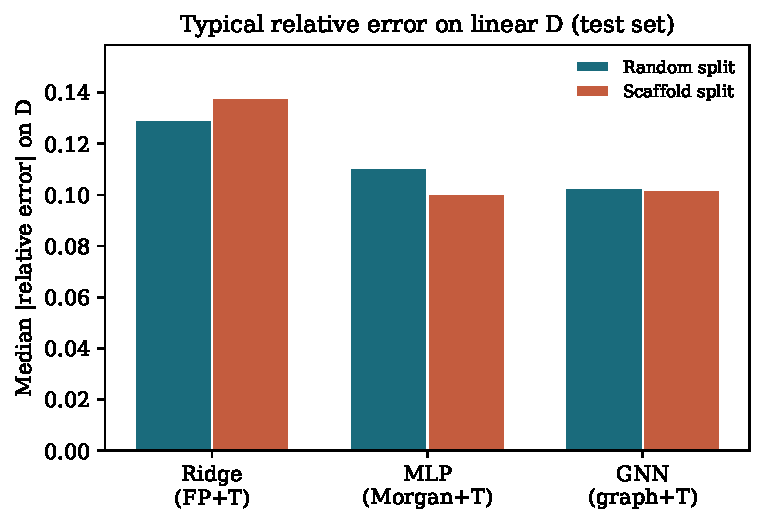
\includegraphics[width=0.75\linewidth]{figures/median_rel_error_D.pdf}
  \caption{Median $\lvert \hat{D}-D\rvert/D$ on the test set (mean/median baselines $\approx 0.77$--$0.79$, not shown).}
  \label{fig:med}
\end{figure}

\section{Discussion}
\subsection{Random versus scaffold test performance}
A large scaffold--random gap would indicate reliance on memorizing chemotypes. In our single-seed run, scaffold metrics were not uniformly worse than random (split variance and dataset structure can produce this). The key takeaway is that \textbf{both} protocols show large margins over trivial baselines; reporting \textbf{both} is still best practice.

\subsection{Limitations}
\begin{itemize}
  \item \textbf{Solvent:} trained for water only.
  \item \textbf{Units:} confirm $D$ units in the primary paper before comparing absolute numbers to other corpora.
  \item \textbf{Extrapolation:} $T$ outside the training range is extrapolation; the inference helper can flag this using stored training bounds.
  \item \textbf{No uncertainty:} point predictions only; no calibrated epistemic intervals.
  \item \textbf{Pretrained SMILES encoders} (e.g.\ ChemBERTa) are natural next steps but not implemented here.
\end{itemize}

\subsection{Optional external comparison}
The same Excel workbook contains \texttt{Table S6} with literature model predictions versus experiment; it can be used as an informal reference but \textbf{not} as a substitute for the held-out protocol above.

\section{Conclusion}
We implemented a reproducible end-to-end workflow from the Han et al.\ Table~S2 spreadsheet to cleaned data, molecule-consistent splits, and neural regressors with sensible baselines. GNN and MLP both achieve strong test performance on $\log_{10} D$; the GNN is slightly ahead in our scaffold run. Future work: uncertainty, pretrained sequence encoders, and explicit unit validation against the primary article.

\appendix
\section{Default hyperparameters}
\label{app:hp}
\begin{table}[ht]
  \centering
  \caption{Values from \texttt{configs/default.yaml} (unless overridden on the command line).}
  \GeneratedHyperparamTable
\end{table}

\begin{thebibliography}{9}
\bibitem{han_si}
Supporting information dataset: \texttt{jp5c01881\_si\_002.xlsx}, sheet \texttt{Table S2}. Associated with J.\ Phys.\ Chem.\ Lett.\ article identifier \texttt{jp5c01881} (ACS). Use the journal landing page for the definitive citation and $D$ unit conventions.
\bibitem{splitting}
J.\ B.\ Brown and T.\ Stergiou, ``Some thoughts on splitting chemical datasets,'' \textit{Practical Cheminformatics} (blog), 2024. Discusses random vs.\ scaffold splits for molecular generalization.
\end{thebibliography}

\end{document}
